\documentclass[14pt]{extbook}
\usepackage{multicol, enumerate, enumitem, hyperref, color, soul, setspace, parskip, fancyhdr} %General Packages
\usepackage{amssymb, amsthm, amsmath, latexsym, units, mathtools} %Math Packages
\everymath{\displaystyle} %All math in Display Style
% Packages with additional options
\usepackage[headsep=0.5cm,headheight=12pt, left=1 in,right= 1 in,top= 1 in,bottom= 1 in]{geometry}
\usepackage[usenames,dvipsnames]{xcolor}
\usepackage{dashrule}  % Package to use the command below to create lines between items
\newcommand{\litem}[1]{\item#1\hspace*{-1cm}\rule{\textwidth}{0.4pt}}
\pagestyle{fancy}
\lhead{Progress Quiz 7}
\chead{}
\rhead{Version ALL}
\lfoot{3510-5252}
\cfoot{}
\rfoot{Summer C 2021}
\begin{document}

\begin{enumerate}
\litem{
For the scenario below, use the model for the volume of a cylinder as $V = \pi r^2 h$.
\begin{center}
    \textit{ Pringles wants to add 50 \text{percent} more chips to their cylinder cans and minimize the design change of their cans. They've decided that the best way to minimize the design change is to increase the radius and height by the same percentage. What should this increase be? }
\end{center}
\begin{enumerate}[label=\Alph*.]
\item \( \text{About } 22 \text{ percent} \)
\item \( \text{About } 14 \text{ percent} \)
\item \( \text{About } 4 \text{ percent} \)
\item \( \text{About } 25 \text{ percent} \)
\item \( \text{None of the above} \)

\end{enumerate} }
\litem{
For the scenario below, use the model for the volume of a cylinder as $V = \pi r^2 h$.
\begin{center}
    \textit{ Pringles wants to add 24 \text{percent} more chips to their cylinder cans and minimize the design change of their cans. They've decided that the best way to minimize the design change is to increase the radius and height by the same percentage. What should this increase be? }
\end{center}
\begin{enumerate}[label=\Alph*.]
\item \( \text{About } 11 \text{ percent} \)
\item \( \text{About } 7 \text{ percent} \)
\item \( \text{About } 12 \text{ percent} \)
\item \( \text{About } 3 \text{ percent} \)
\item \( \text{None of the above} \)

\end{enumerate} }
\litem{
Determine the appropriate model for the graph of points below.
\begin{center}
    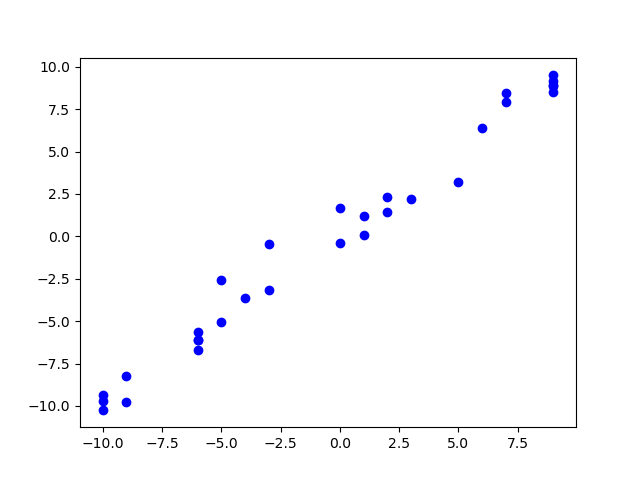
\includegraphics[width=0.5\textwidth]{../Figures/identifyModelGraph12CopyA.png}
\end{center}
\begin{enumerate}[label=\Alph*.]
\item \( \text{Exponential model} \)
\item \( \text{Linear model} \)
\item \( \text{Logarithmic model} \)
\item \( \text{Non-linear Power model} \)
\item \( \text{None of the above} \)

\end{enumerate} }
\litem{
Solve the modeling problem below, if possible.
\begin{center}
    \textit{ A new virus is spreading throughout the world. There were initially 3 many cases reported, but the number of confirmed cases has doubled every 1 days. How long will it be until there are at least 1000000 confirmed cases? }
\end{center}
\begin{enumerate}[label=\Alph*.]
\item \( \text{About } 19 \text{ days} \)
\item \( \text{About } 8 \text{ days} \)
\item \( \text{About } 7 \text{ days} \)
\item \( \text{About } 13 \text{ days} \)
\item \( \text{There is not enough information to solve the problem.} \)

\end{enumerate} }
\litem{
Solve the modeling problem below, if possible.
\begin{center}
    \textit{ In CHM2045L, Brittany created a 29 liter 15 percent solution of chemical $\chi$ using two different solution percentages of chemical $\chi$. When she went to write her lab report, she realized she forgot to write the amount of each solution she used! If she remembers she used 15 percent and 35 percent solutions, what was the amount she used of the 35 percent solution? }
\end{center}
\begin{enumerate}[label=\Alph*.]
\item \( 0.00 liters \)
\item \( 29.00 liters \)
\item \( 14.50 liters \)
\item \( 1.29 liters \)
\item \( \text{There is not enough information to solve the problem.} \)

\end{enumerate} }
\litem{
Using the situation below, construct a linear model that describes the cost of the coffee beans $C(h)$ in terms of the weight of the high-quality coffee beans $h$.
\begin{center}
    \textit{ Veronica needs to prepare 220 of blended coffee beans selling for \$3.06 per pound. She has a high-quality bean that sells for \$4.31 a pound and a low-quality bean that sells for \$2.47 a pound. }
\end{center}
\begin{enumerate}[label=\Alph*.]
\item \( C(h) = -1.84 h + 948.20 \)
\item \( C(h) = 4.31 h \)
\item \( C(h) = 3.39 h \)
\item \( C(h) = 1.84 h + 543.40 \)
\item \( \text{None of the above.} \)

\end{enumerate} }
\litem{
For the information below, construct a linear model that describes the total time $T$ spent on the path in terms of the distance of a particular part of the path \textit{if we know that all parts of the path are equal length}.
\begin{center}
    \textit{ A bicyclist is training for a race on a hilly path. Their bike keeps track of their speed at any time, but not the distance traveled. Their speed traveling up a hill is 7 mph, 10 mph when traveling down a hill, and 8 mph when traveling along a flat portion. }
\end{center}
\begin{enumerate}[label=\Alph*.]
\item \( 0.368 D \)
\item \( 25.000 D \)
\item \( 560.000 D \)
\item \( \text{The model can be found with the information provided, but isn't options 1-3.} \)
\item \( \text{The model cannot be found with the information provided.} \)

\end{enumerate} }
\litem{
Determine the appropriate model for the graph of points below.
\begin{center}
    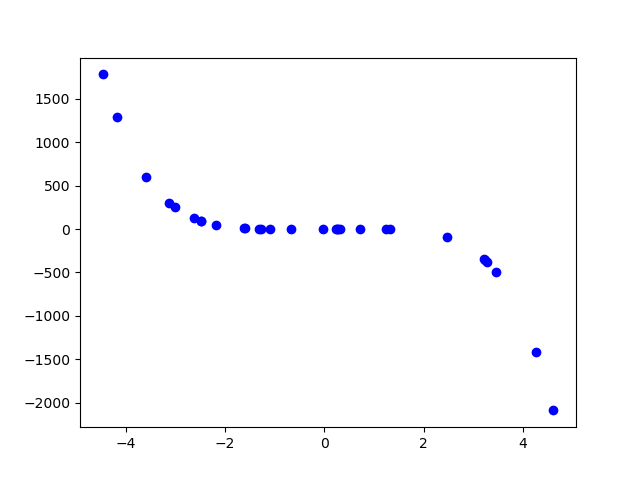
\includegraphics[width=0.5\textwidth]{../Figures/identifyModelGraph12A.png}
\end{center}
\begin{enumerate}[label=\Alph*.]
\item \( \text{Exponential model} \)
\item \( \text{Linear model} \)
\item \( \text{Logarithmic model} \)
\item \( \text{Non-linear Power model} \)
\item \( \text{None of the above} \)

\end{enumerate} }
\litem{
Solve the modeling problem below, if possible.
\begin{center}
    \textit{ A new virus is spreading throughout the world. There were initially 8 many cases reported, but the number of confirmed cases has quadrupled every 5 days. How long will it be until there are at least 1000 confirmed cases? }
\end{center}
\begin{enumerate}[label=\Alph*.]
\item \( \text{About } 18 \text{ days} \)
\item \( \text{About } 12 \text{ days} \)
\item \( \text{About } 25 \text{ days} \)
\item \( \text{About } 10 \text{ days} \)
\item \( \text{There is not enough information to solve the problem.} \)

\end{enumerate} }
\litem{
Solve the modeling problem below, if possible.
\begin{center}
    \textit{ In CHM2045L, Brittany created a 22 liter 26 percent solution of chemical $\chi$ using two different solution percentages of chemical $\chi$. When she went to write her lab report, she realized she forgot to write the amount of each solution she used! If she remembers she used 7 percent and 31 percent solutions, what was the amount she used of the 31 percent solution? }
\end{center}
\begin{enumerate}[label=\Alph*.]
\item \( 16.81 liters \)
\item \( 17.42 liters \)
\item \( 4.58 liters \)
\item \( 11.00 liters \)
\item \( \text{There is not enough information to solve the problem.} \)

\end{enumerate} }
\litem{
For the scenario below, use the model for the volume of a cylinder as $V = \pi r^2 h$.
\begin{center}
    \textit{ Pringles wants to add 35 \text{percent} more chips to their cylinder cans and minimize the design change of their cans. They've decided that the best way to minimize the design change is to increase the radius and height by the same percentage. What should this increase be? }
\end{center}
\begin{enumerate}[label=\Alph*.]
\item \( \text{About } 16 \text{ percent} \)
\item \( \text{About } 3 \text{ percent} \)
\item \( \text{About } 11 \text{ percent} \)
\item \( \text{About } 18 \text{ percent} \)
\item \( \text{None of the above} \)

\end{enumerate} }
\litem{
For the scenario below, use the model for the volume of a cylinder as $V = \pi r^2 h$.
\begin{center}
    \textit{ Pringles wants to add 24 \text{percent} more chips to their cylinder cans and minimize the design change of their cans. They've decided that the best way to minimize the design change is to increase the radius and height by the same percentage. What should this increase be? }
\end{center}
\begin{enumerate}[label=\Alph*.]
\item \( \text{About } 11 \text{ percent} \)
\item \( \text{About } 3 \text{ percent} \)
\item \( \text{About } 12 \text{ percent} \)
\item \( \text{About } 7 \text{ percent} \)
\item \( \text{None of the above} \)

\end{enumerate} }
\litem{
Determine the appropriate model for the graph of points below.
\begin{center}
    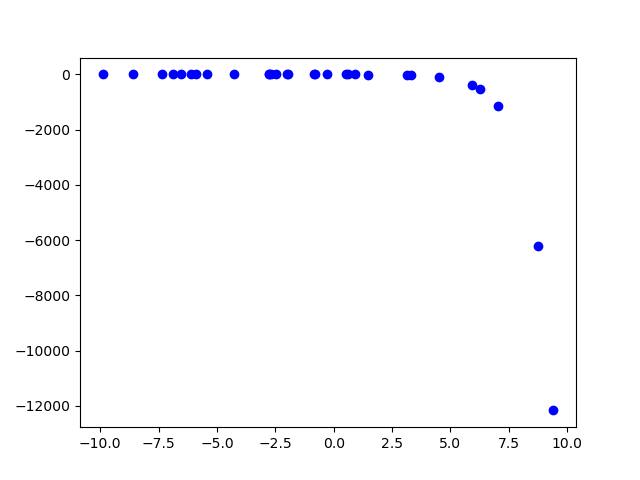
\includegraphics[width=0.5\textwidth]{../Figures/identifyModelGraph12CopyB.png}
\end{center}
\begin{enumerate}[label=\Alph*.]
\item \( \text{Exponential model} \)
\item \( \text{Non-linear Power model} \)
\item \( \text{Logarithmic model} \)
\item \( \text{Linear model} \)
\item \( \text{None of the above} \)

\end{enumerate} }
\litem{
Solve the modeling problem below, if possible.
\begin{center}
    \textit{ A new virus is spreading throughout the world. There were initially 8 many cases reported, but the number of confirmed cases has doubled every 3 days. How long will it be until there are at least 100000 confirmed cases? }
\end{center}
\begin{enumerate}[label=\Alph*.]
\item \( \text{About } 41 \text{ days} \)
\item \( \text{About } 29 \text{ days} \)
\item \( \text{About } 12 \text{ days} \)
\item \( \text{About } 13 \text{ days} \)
\item \( \text{There is not enough information to solve the problem.} \)

\end{enumerate} }
\litem{
Solve the modeling problem below, if possible.
\begin{center}
    \textit{ In CHM2045L, Brittany created a 23 liter 11 percent solution of chemical $\chi$ using two different solution percentages of chemical $\chi$. When she went to write her lab report, she realized she forgot to write the amount of each solution she used! If she remembers she used 9 percent and 22 percent solutions, what was the amount she used of the 22 percent solution? }
\end{center}
\begin{enumerate}[label=\Alph*.]
\item \( 3.54 liters \)
\item \( 11.50 liters \)
\item \( 19.46 liters \)
\item \( 7.88 liters \)
\item \( \text{There is not enough information to solve the problem.} \)

\end{enumerate} }
\litem{
For the scenario below, find the variation constant $k$ of the model (if possible).
\begin{center}
    \textit{ In an alternative galaxy, the quartic of the time, $T$ (Earth years), required for a planet to orbit Sun $\chi$ decreases as the square of the distance, $d$ (AUs), that the planet is from Sun $\chi$ decreases. For example, when Ea's average distance from Sun $\chi$ is 8, it takes 89 Earth days to complete an orbit. }
\end{center}
\begin{enumerate}[label=\Alph*.]
\item \( k = 980347.516 \)
\item \( k = 4.028 \)
\item \( k = 4015503424.000 \)
\item \( k = 1.086 \)
\item \( \text{Unable to compute the constant based on the information given.} \)

\end{enumerate} }
\litem{
Using the situation below, construct a linear model that describes the cost of the coffee beans $C(h)$ in terms of the weight of the low-quality coffee beans $h$.
\begin{center}
    \textit{ Veronica needs to prepare 120 of blended coffee beans selling for \$6.11 per pound. She has a high-quality bean that sells for \$7.57 a pound and a low-quality bean that sells for \$4.86 a pound. }
\end{center}
\begin{enumerate}[label=\Alph*.]
\item \( C(h) = 6.21 h \)
\item \( C(h) = 2.71 h + 583.20 \)
\item \( C(h) = -2.71 h + 908.40 \)
\item \( C(h) = 4.86 h \)
\item \( \text{None of the above.} \)

\end{enumerate} }
\litem{
Determine the appropriate model for the graph of points below.
\begin{center}
    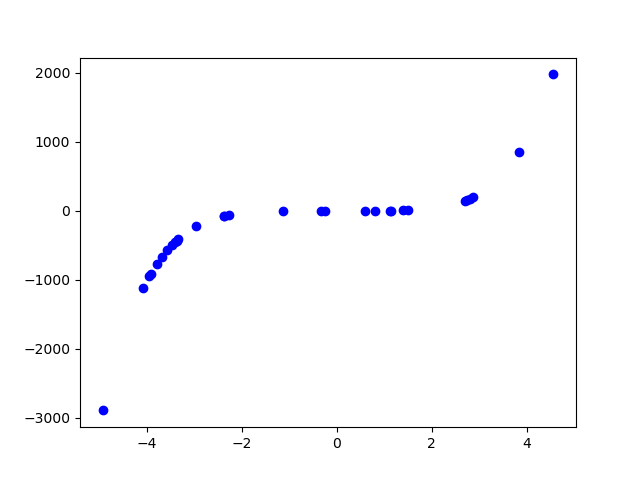
\includegraphics[width=0.5\textwidth]{../Figures/identifyModelGraph12B.png}
\end{center}
\begin{enumerate}[label=\Alph*.]
\item \( \text{Logarithmic model} \)
\item \( \text{Linear model} \)
\item \( \text{Non-linear Power model} \)
\item \( \text{Exponential model} \)
\item \( \text{None of the above} \)

\end{enumerate} }
\litem{
Solve the modeling problem below, if possible.
\begin{center}
    \textit{ A new virus is spreading throughout the world. There were initially 5 many cases reported, but the number of confirmed cases has quadrupled every 3 days. How long will it be until there are at least 10000 confirmed cases? }
\end{center}
\begin{enumerate}[label=\Alph*.]
\item \( \text{About } 23 \text{ days} \)
\item \( \text{About } 10 \text{ days} \)
\item \( \text{About } 17 \text{ days} \)
\item \( \text{About } 11 \text{ days} \)
\item \( \text{There is not enough information to solve the problem.} \)

\end{enumerate} }
\litem{
Solve the modeling problem below, if possible.
\begin{center}
    \textit{ In CHM2045L, Brittany created a 29 liter 27 percent solution of chemical $\chi$ using two different solution percentages of chemical $\chi$. When she went to write her lab report, she realized she forgot to write the amount of each solution she used! If she remembers she used 17 percent and 39 percent solutions, what was the amount she used of the 39 percent solution? }
\end{center}
\begin{enumerate}[label=\Alph*.]
\item \( 13.63 liters \)
\item \( 14.50 liters \)
\item \( 15.82 liters \)
\item \( 13.18 liters \)
\item \( \text{There is not enough information to solve the problem.} \)

\end{enumerate} }
\litem{
For the scenario below, use the model for the volume of a cylinder as $V = \pi r^2 h$.
\begin{center}
    \textit{ Pringles wants to add 27 \text{percent} more chips to their cylinder cans and minimize the design change of their cans. They've decided that the best way to minimize the design change is to increase the radius and height by the same percentage. What should this increase be? }
\end{center}
\begin{enumerate}[label=\Alph*.]
\item \( \text{About } 13 \text{ percent} \)
\item \( \text{About } 8 \text{ percent} \)
\item \( \text{About } 3 \text{ percent} \)
\item \( \text{About } 14 \text{ percent} \)
\item \( \text{None of the above} \)

\end{enumerate} }
\litem{
For the scenario below, use the model for the volume of a cylinder as $V = \pi r^2 h$.
\begin{center}
    \textit{ Pringles wants to add 38 \text{percent} more chips to their cylinder cans and minimize the design change of their cans. They've decided that the best way to minimize the design change is to increase the radius and height by the same percentage. What should this increase be? }
\end{center}
\begin{enumerate}[label=\Alph*.]
\item \( \text{About } 3 \text{ percent} \)
\item \( \text{About } 11 \text{ percent} \)
\item \( \text{About } 19 \text{ percent} \)
\item \( \text{About } 17 \text{ percent} \)
\item \( \text{None of the above} \)

\end{enumerate} }
\litem{
Determine the appropriate model for the graph of points below.
\begin{center}
    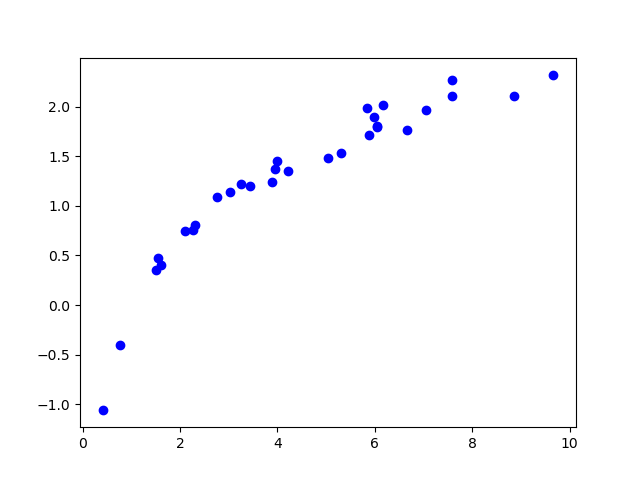
\includegraphics[width=0.5\textwidth]{../Figures/identifyModelGraph12CopyC.png}
\end{center}
\begin{enumerate}[label=\Alph*.]
\item \( \text{Logarithmic model} \)
\item \( \text{Non-linear Power model} \)
\item \( \text{Linear model} \)
\item \( \text{Exponential model} \)
\item \( \text{None of the above} \)

\end{enumerate} }
\litem{
Solve the modeling problem below, if possible.
\begin{center}
    \textit{ A new virus is spreading throughout the world. There were initially 3 many cases reported, but the number of confirmed cases has doubled every 4 days. How long will it be until there are at least 1000 confirmed cases? }
\end{center}
\begin{enumerate}[label=\Alph*.]
\item \( \text{About } 34 \text{ days} \)
\item \( \text{About } 14 \text{ days} \)
\item \( \text{About } 24 \text{ days} \)
\item \( \text{About } 16 \text{ days} \)
\item \( \text{There is not enough information to solve the problem.} \)

\end{enumerate} }
\litem{
Solve the modeling problem below, if possible.
\begin{center}
    \textit{ In CHM2045L, Brittany created a 26 liter 31 percent solution of chemical $\chi$ using two different solution percentages of chemical $\chi$. When she went to write her lab report, she realized she forgot to write the amount of each solution she used! If she remembers she used 20 percent and 50 percent solutions, what was the amount she used of the 20 percent solution? }
\end{center}
\begin{enumerate}[label=\Alph*.]
\item \( 9.53 liters \)
\item \( 16.47 liters \)
\item \( 11.85 liters \)
\item \( 13.00 liters \)
\item \( \text{There is not enough information to solve the problem.} \)

\end{enumerate} }
\litem{
The temperature of an object, $T$, in a different surrounding temperature $T_s$ will behave according to the formula $T(t) = Ae^{kt} + T_s$, where $t$ is minutes, $A$ is a constant, and k is a constant. Use this formula and the situation below to construct a model that describes the uranium's temperature, $T$, based on the amount of time t (in minutes) that have passed. Choose the correct constant $k$ from the options below.
\begin{center}
    \textit{ Uranium is taken out of the reactor with a temperature of $130^{\circ}$ C and is placed into a $16^{\circ}$ C bath to cool. After 40 minutes, the uranium has cooled to $63^{\circ}$ C. }
\end{center}
\begin{enumerate}[label=\Alph*.]
\item \( k = -0.02551 \)
\item \( k = -0.02543 \)
\item \( k = -0.01678 \)
\item \( k = -0.01640 \)
\item \( \text{None of the above} \)

\end{enumerate} }
\litem{
Using the situation below, construct a linear model that describes the cost of the coffee beans $C(h)$ in terms of the weight of the low-quality coffee beans $h$.
\begin{center}
    \textit{ Veronica needs to prepare 130 of blended coffee beans selling for \$2.77 per pound. She has a high-quality bean that sells for \$3.28 a pound and a low-quality bean that sells for \$2.21 a pound. }
\end{center}
\begin{enumerate}[label=\Alph*.]
\item \( C(h) = 2.21 h \)
\item \( C(h) = -1.07 h + 426.40 \)
\item \( C(h) = 2.75 h \)
\item \( C(h) = 1.07 h + 287.30 \)
\item \( \text{None of the above.} \)

\end{enumerate} }
\litem{
Determine the appropriate model for the graph of points below.
\begin{center}
    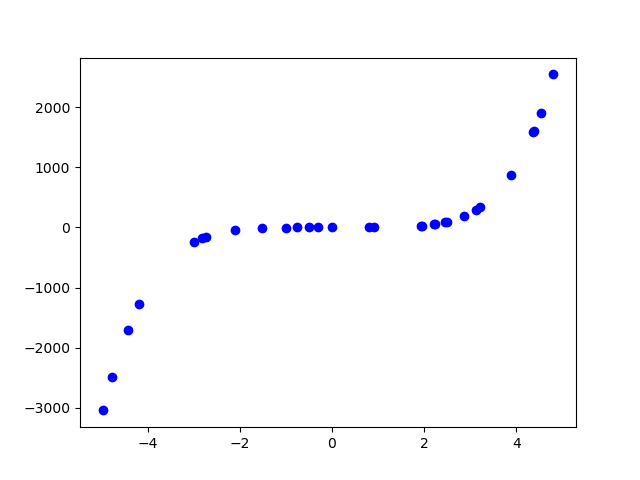
\includegraphics[width=0.5\textwidth]{../Figures/identifyModelGraph12C.png}
\end{center}
\begin{enumerate}[label=\Alph*.]
\item \( \text{Non-linear Power model} \)
\item \( \text{Linear model} \)
\item \( \text{Exponential model} \)
\item \( \text{Logarithmic model} \)
\item \( \text{None of the above} \)

\end{enumerate} }
\litem{
Solve the modeling problem below, if possible.
\begin{center}
    \textit{ A new virus is spreading throughout the world. There were initially 6 many cases reported, but the number of confirmed cases has doubled every 3 days. How long will it be until there are at least 10000 confirmed cases? }
\end{center}
\begin{enumerate}[label=\Alph*.]
\item \( \text{About } 10 \text{ days} \)
\item \( \text{About } 23 \text{ days} \)
\item \( \text{About } 33 \text{ days} \)
\item \( \text{About } 12 \text{ days} \)
\item \( \text{There is not enough information to solve the problem.} \)

\end{enumerate} }
\litem{
Solve the modeling problem below, if possible.
\begin{center}
    \textit{ In CHM2045L, Brittany created a 18 liter 18 percent solution of chemical $\chi$ using two different solution percentages of chemical $\chi$. When she went to write her lab report, she realized she forgot to write the amount of each solution she used! If she remembers she used 16 percent and 45 percent solutions, what was the amount she used of the 45 percent solution? }
\end{center}
\begin{enumerate}[label=\Alph*.]
\item \( 14.98 liters \)
\item \( 1.24 liters \)
\item \( 16.76 liters \)
\item \( 9.00 liters \)
\item \( \text{There is not enough information to solve the problem.} \)

\end{enumerate} }
\end{enumerate}

\end{document}